% !TeX spellcheck = en_US
\documentclass[french]{article}
\usepackage[T1]{fontenc}
\usepackage[utf8]{inputenc}
\usepackage{lmodern}
\usepackage[a4paper]{geometry}
\usepackage{babel}
\usepackage{graphicx}

\begin{document}
\title{Nuages de points et modélisation 3D\\
TP 3 : Neighborhood descriptors}
\author{Marius Dufraisse}
\date{}

\maketitle


\paragraph{Question 1.} When the radius is too big small details do not appear in the computed normal map. For instance borders of the windows can be seen when the radius is equal to 50cm (see Figure \ref{fig:q1-50cm}) but when the radius is equal to 5m the wall is in a single color (see Figure \ref{fig:q1-5m}).

When the radius is too small, noise in the data results in noise in the normal (see Figure \ref{fig:q1-5cm} for results with a 5cm radius).



\begin{figure}[h]
	\centering
	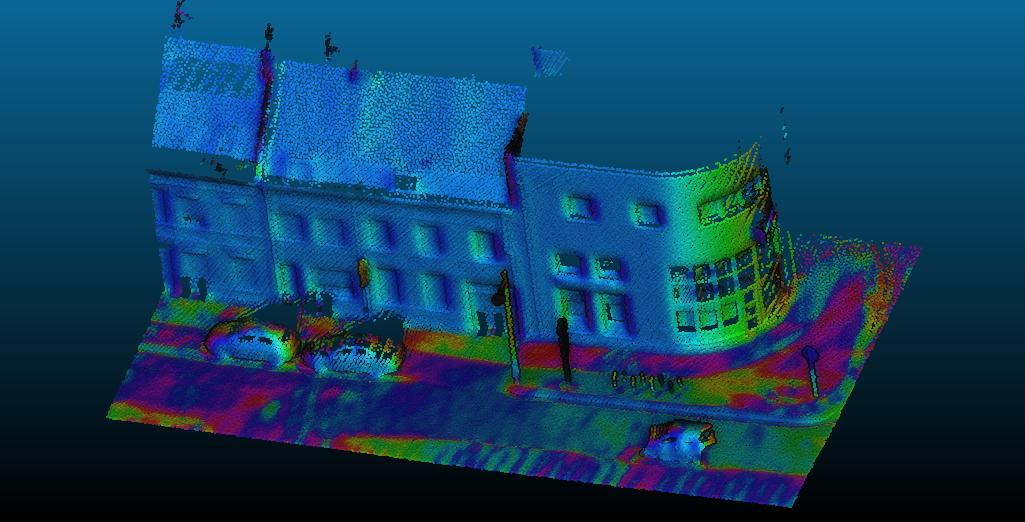
\includegraphics[width=0.6\linewidth]{q1-r50cm.jpg}
	\caption{Normals obtained with a radius of 50cm.}
	\label{fig:q1-50cm}
\end{figure}

\begin{figure}[h]
	\centering
	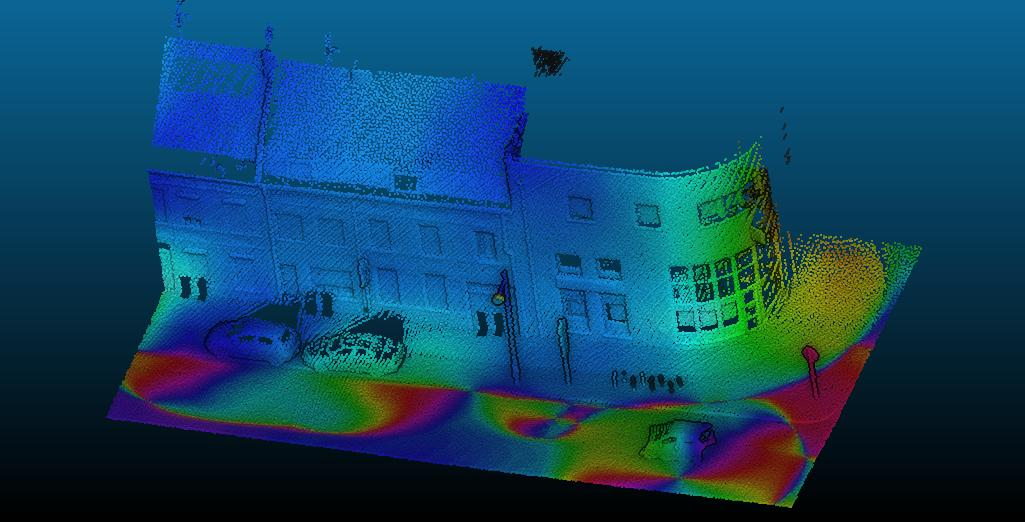
\includegraphics[width=0.6\linewidth]{q1-r5m.jpg}
	\caption{Normals obtained with a radius of 5m.}
	\label{fig:q1-5m}
\end{figure}

\begin{figure}[h]
	\centering
	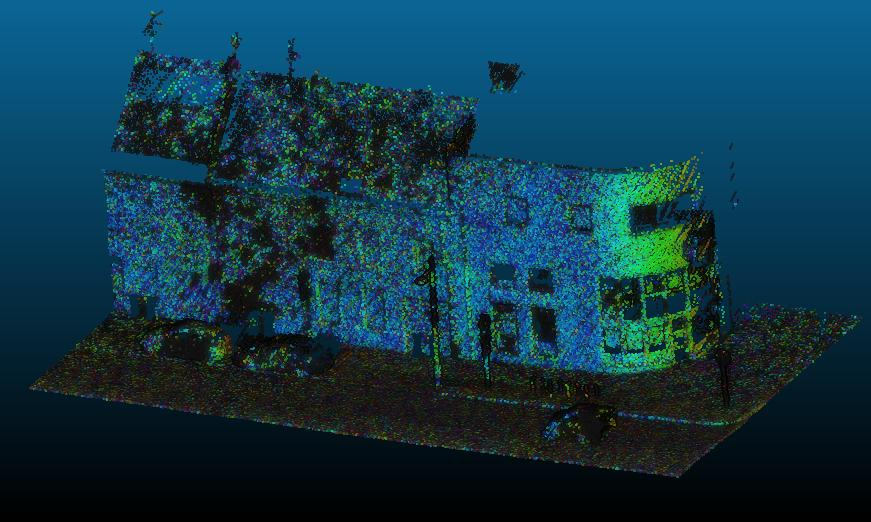
\includegraphics[width=0.6\linewidth]{q1-r5cm.jpg}
	\caption{Normals obtained with a radius of 5cm.}
	\label{fig:q1-5cm}
\end{figure}

\paragraph{Question 2.} A good way to choose the radius would be to take it as small as the biggest detail we want to analyze. However, I have no idea how this could be computed using just the point cloud.

\paragraph{Question 3.} My results are shown in Figure \ref{fig:q3}. In order to have normal oriented in the same direction I compared the computed normal direction to a fixed vector. This was not enough to get normals from every part of the image in the same direction : CloudCompare provides algorithms that solved this issue.

\begin{figure}[h]
	\centering
	\begin{minipage}{0.49\linewidth}
		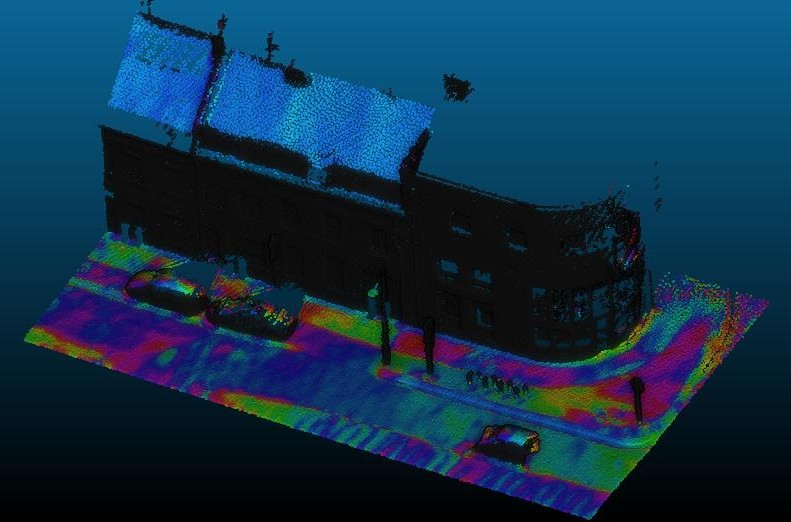
\includegraphics[width=\linewidth]{q3-raw.jpg}
	\end{minipage}\hfill
	\begin{minipage}{0.49\linewidth}
		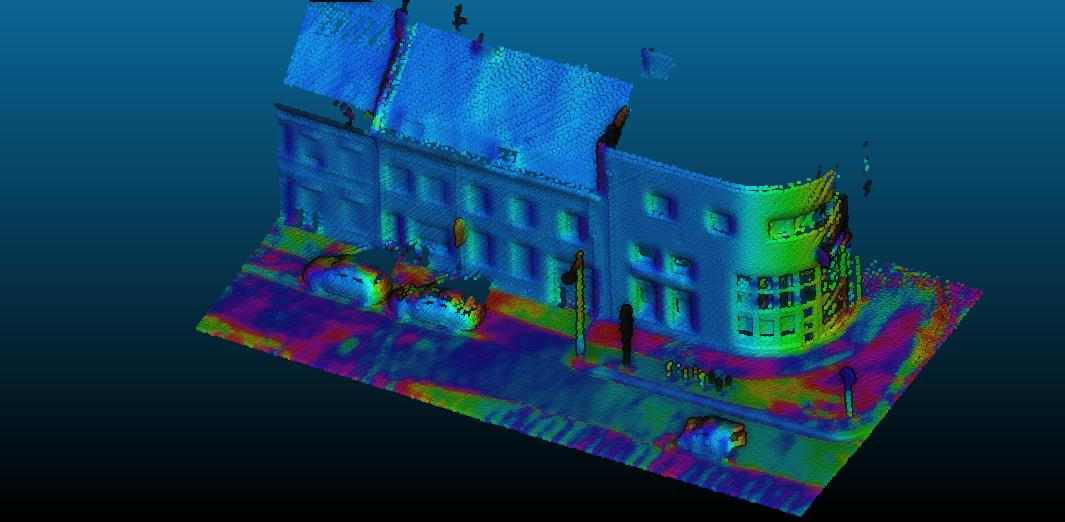
\includegraphics[width=\linewidth]{q3-cheat.jpg}
	\end{minipage}
	\caption{On the left, the normal converted to dip I obtained when trying to align them with a reference vector. On the right, the same normals only using ClouCompare to orient them.}
	\label{fig:q3}
\end{figure}


\paragraph{Question 4.} We can use the smallest eigenvalue as an estimator of the normal estimation quality as it gives an estimation of the diffusion of points in the direction of the normal and thus whether the plan hypothesis is right or not. Figure \ref{fig:q4} display the value of $\lambda_3$ on the point cloud. It is at is the highest on corners were the plan modelisation  is unlikely to estimate normals properly.

\begin{figure}[h]
	\centering
	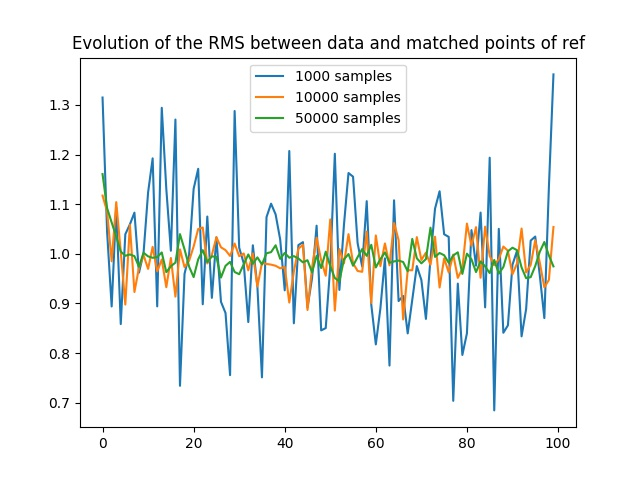
\includegraphics[width=0.6\linewidth]{q4.jpg}
	\caption{Point cloud, the scalar label represents the small eigenvalue.}
	\label{fig:q4}
\end{figure}


\paragraph{Question 5.} 
Screenshot of the 4 features are displayed in Figure \ref{fig:q5}. $linearity$ is equal to $\frac{\lambda_1-\lambda_2}{\lambda_1}$ it measures the diffusion along the second most important axis compared to the first one and thus if points are along one axis. $planarity$ measures if there are points along the third PCA axis and thus if data is along a plan or not. If $sphericity$ is high, $\lambda_1\approx\lambda_3$ meaning that points are not distributed along a specific direction but rather in a sphere.
\begin{figure}[h]
	\centering
	\begin{minipage}{0.49\linewidth}
		\centering
		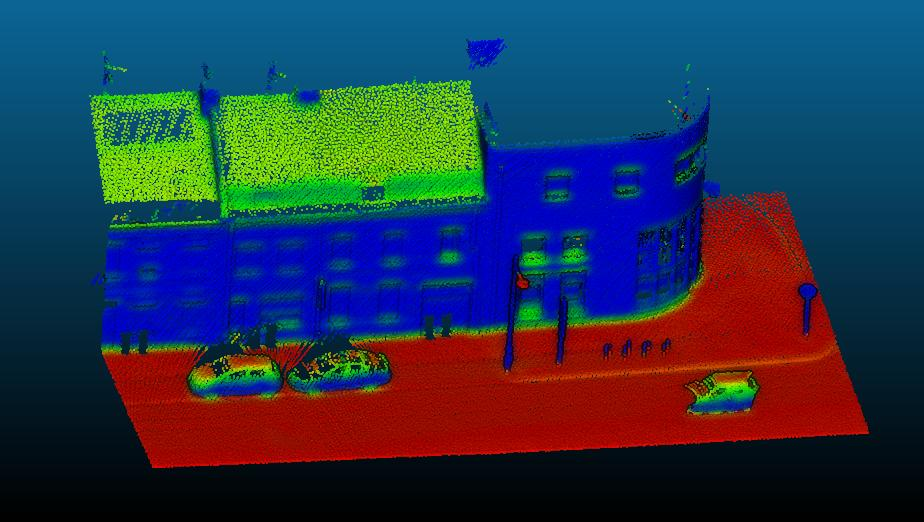
\includegraphics[width=\linewidth]{q5-vert.jpg}
		\textit{Vert}
	\end{minipage}\hfill
	\begin{minipage}{0.49\linewidth}
		\centering
		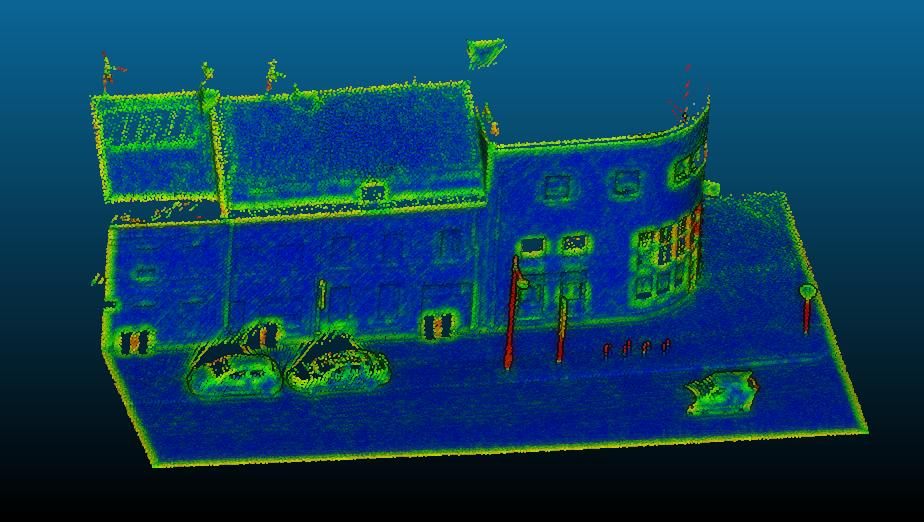
\includegraphics[width=\linewidth]{q5-lin.jpg}
		\textit{Lin}
	\end{minipage}\\

		\begin{minipage}{0.49\linewidth}
		\centering
		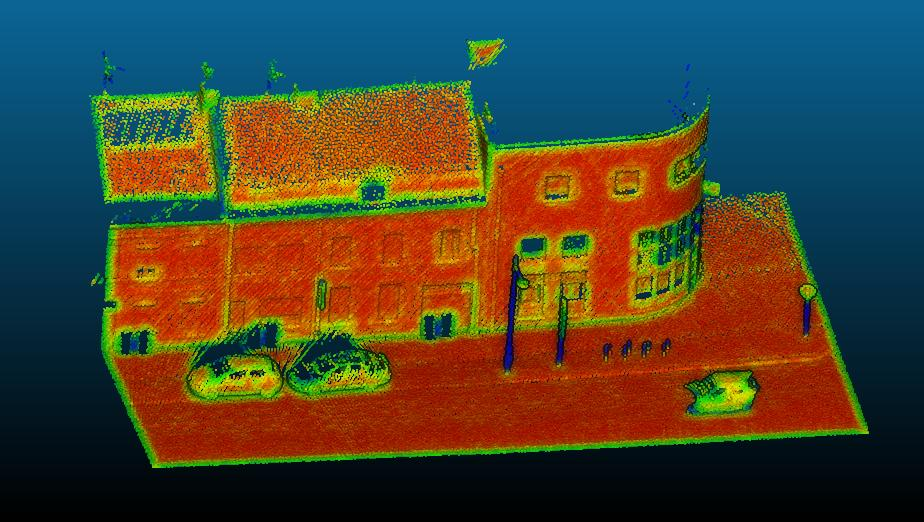
\includegraphics[width=\linewidth]{q5-plan.jpg}
		\textit{Plan}
	\end{minipage}\hfill
	\begin{minipage}{0.49\linewidth}
		\centering
		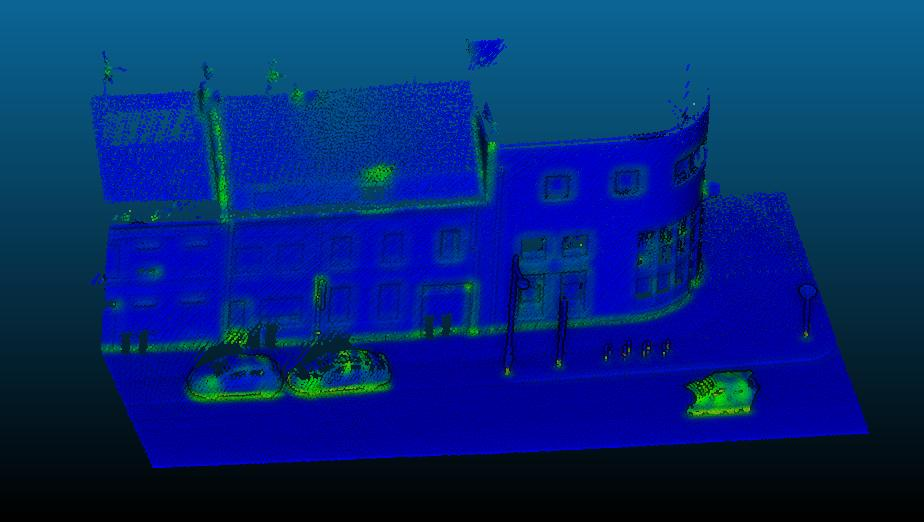
\includegraphics[width=\linewidth]{q5-spher.jpg}
		\textit{Spher}
	\end{minipage}
	\caption{Point clouds colored using the 4 computed indicators.}
	\label{fig:q5}
\end{figure}


\end{document}
